\chapter{Исследовательский раздел}
\label{cha:research}

В данном разделе привидены и проанализированы примеры работы реализованной программы.


Исследования проводились на компьютере следующей конфигурации:
- процессор Intel Core i7-7700 2.80 GHz, 4 логических ядра;
– ОЗУ 8Гб;
– ОС Ubuntu 18.04.
\section{Примеры работы}

На рисунках 4.1, 4.2, 4.3 показана работа программы с различными входными данными.


\begin{figure}[H]
\centering
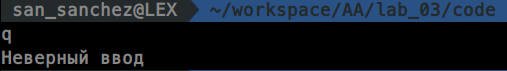
\includegraphics[scale=0.75]{./pictures/wrk2.png}
\caption{Тест на неверный ввод}
\end{figure}
\begin{figure}[H]
\centering
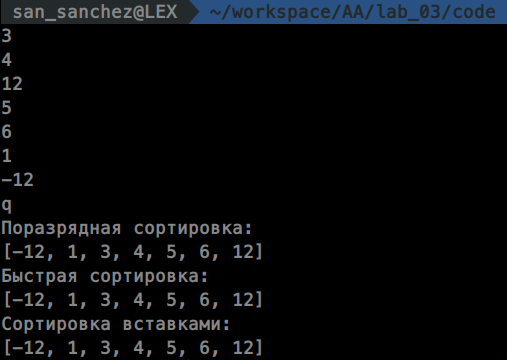
\includegraphics[scale=0.75]{./pictures/wrk3.png}
\caption{Тест на верных входных данных}
\end{figure}
\begin{figure}[H]
\centering
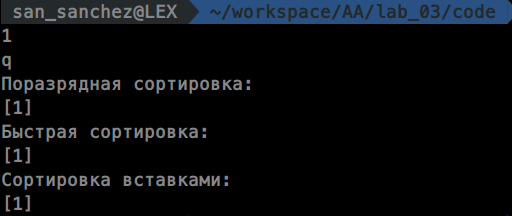
\includegraphics[scale=0.75]{./pictures/wrk5.png}
\caption{Тест при вводе всего одного элемента}
\end{figure}

\newpage
\section{Эксперименты по замеру времени}
На графиках 6-7 представлено сравнение алгоритмов умножения матриц. 
	\begin{center}
        		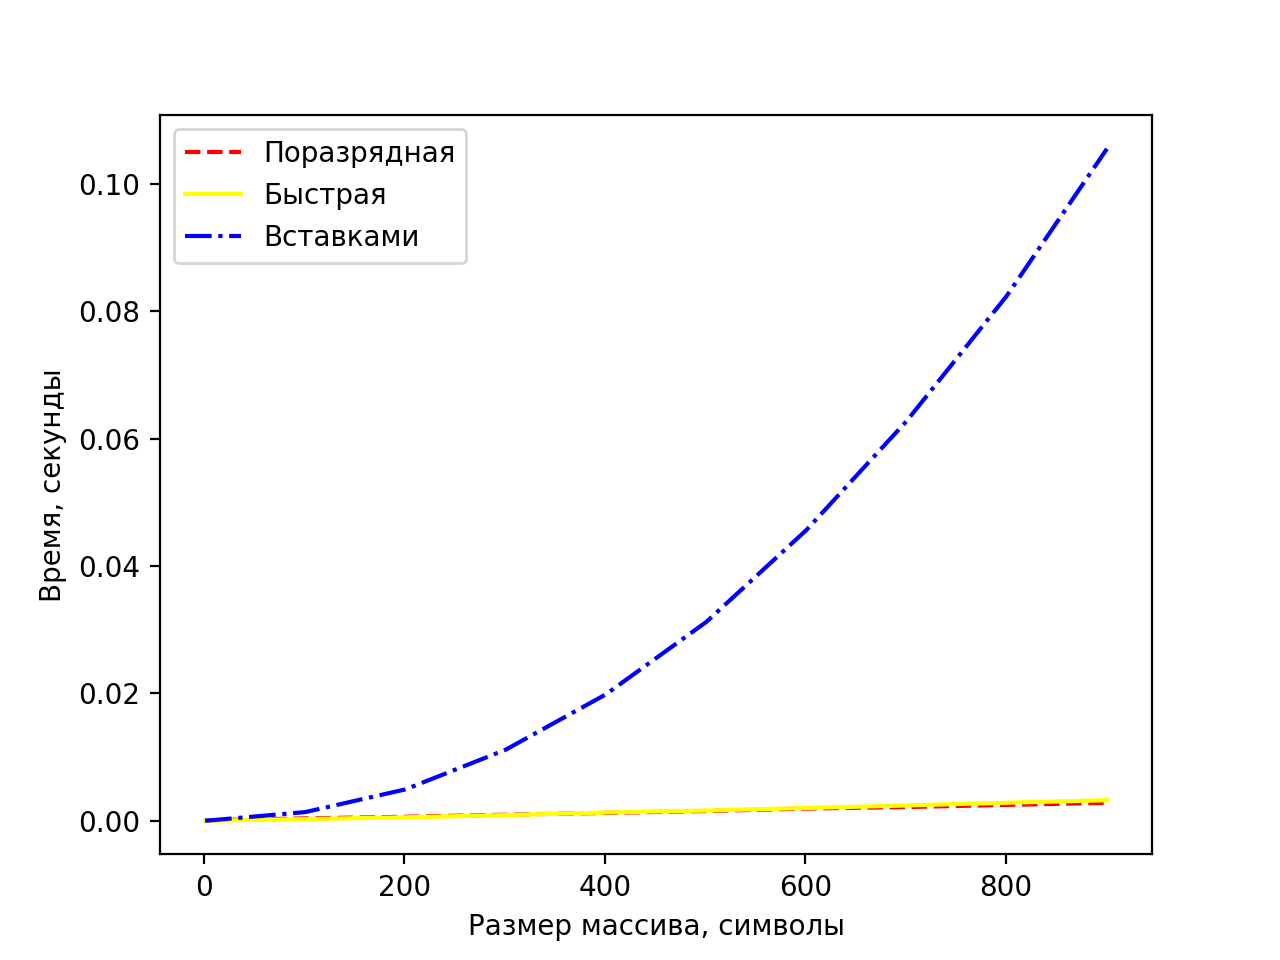
\includegraphics[scale = 1]{./pictures/graph1} \\ Рис. 4.4 - Сравнение реализации алгоритмов сортировок на произвольных данных.
	\end{center}
	
	\begin{center}
        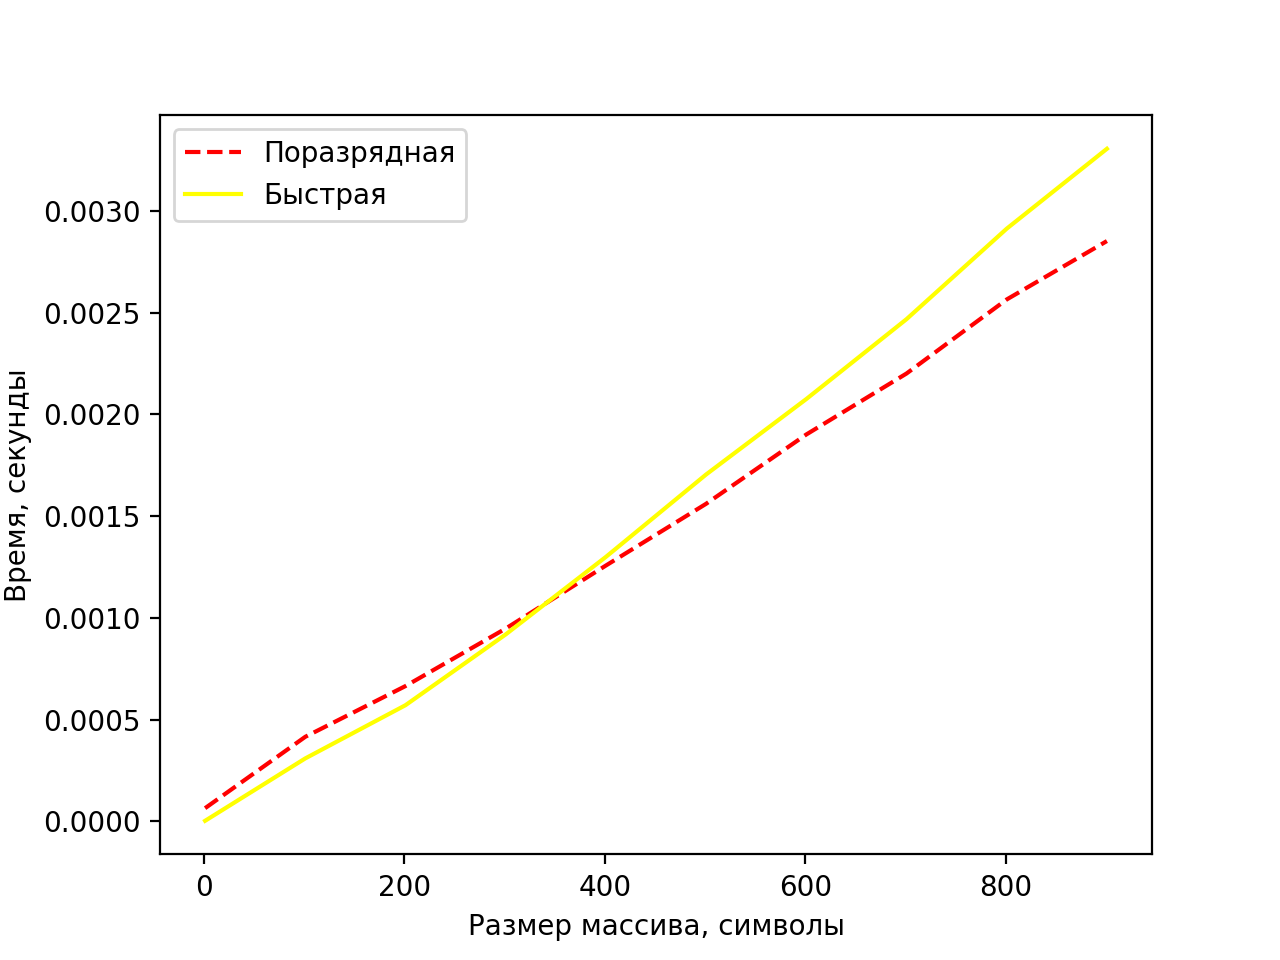
\includegraphics[scale = 1]{./pictures/graph2} \\ Рис. 4.5 - Сравнение реализации алгоритмов сортировок быстрой и поразрядной на произвольных данных(при
        средней разрядности числа до 4 значащих цифр).
	\end{center}
	\begin{center}
        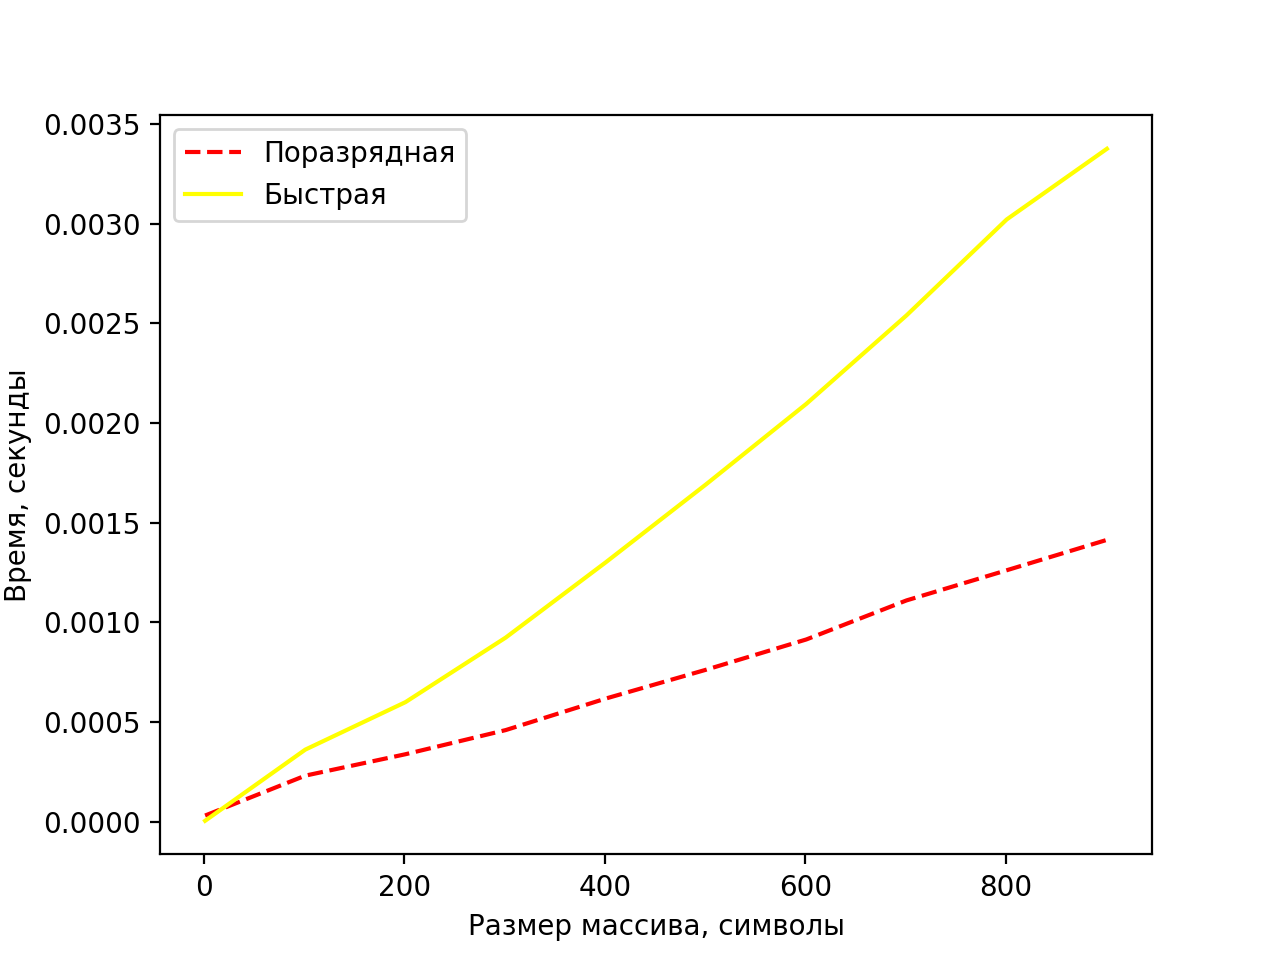
\includegraphics[scale = 1]{./pictures/graph3} \\ Рис. 4.6 - Сравнение реализации алгоритмов сортировок быстрой и поразрядной на произвольных данных (при
        маленькой разрядности числа 1 значащая цифра).
	\end{center}
	\begin{center}
        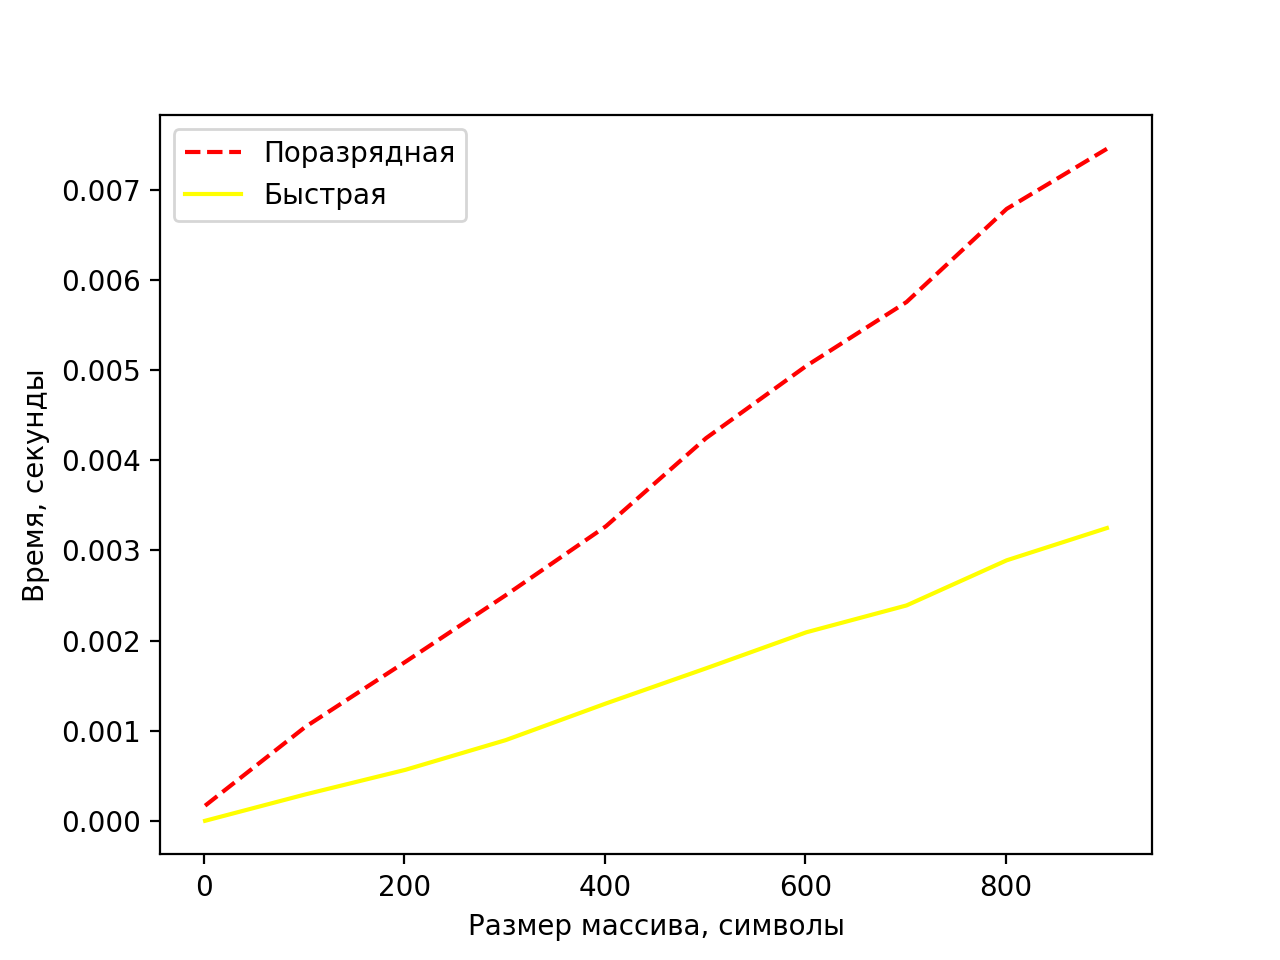
\includegraphics[scale = 1]{./pictures/graph4} \\ Рис. 4.7 - Сравнение реализации алгоритмов сортировок быстрой и поразрядной на произвольных данных (при
        большой разрядности числа до 10 значащих цифр).
	\end{center}
	\begin{center}
        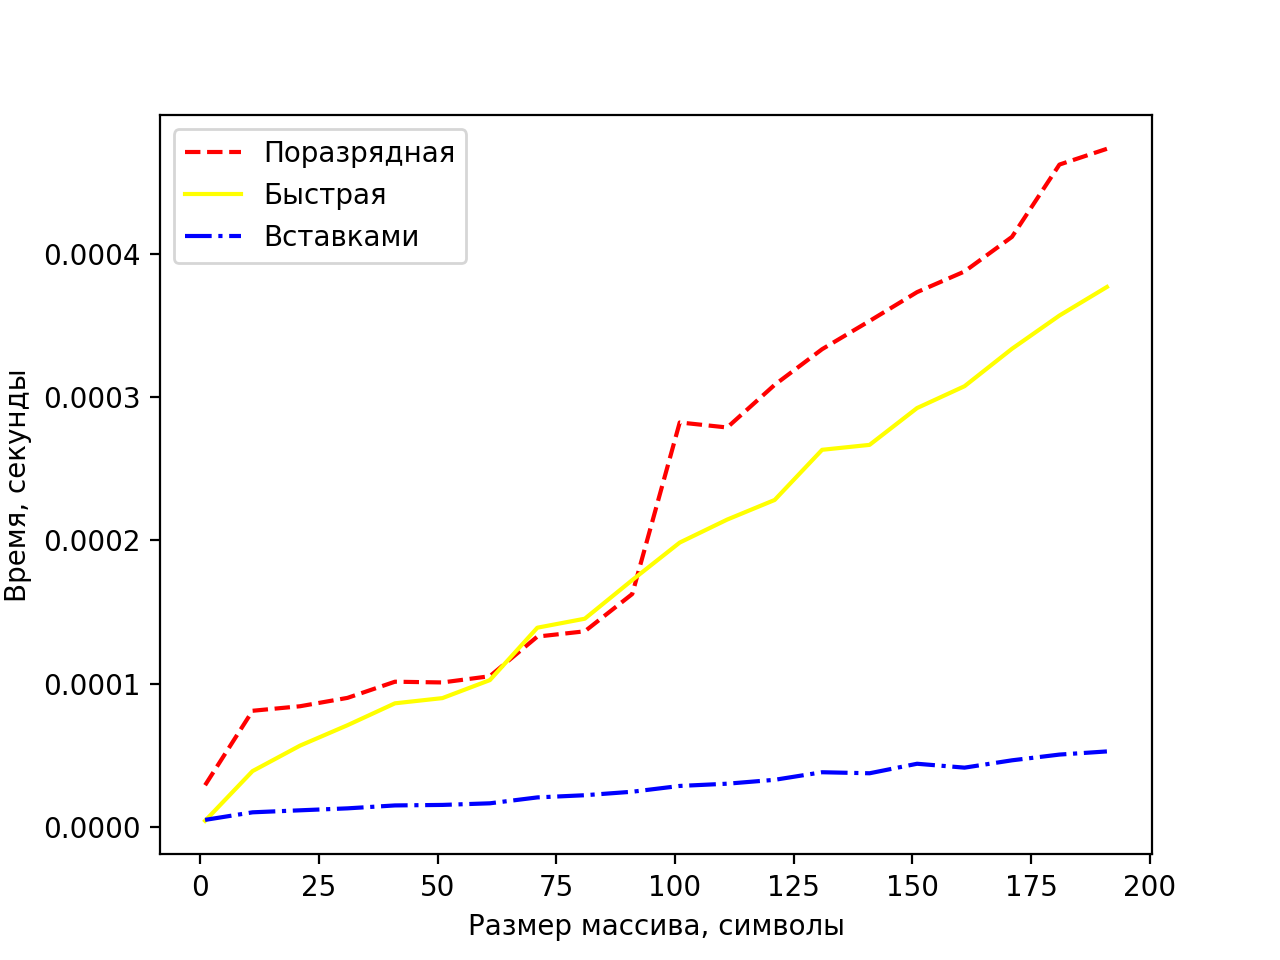
\includegraphics[scale = 1]{./pictures/graph5} \\ Рис. 4.8 - Сравнение реализации алгоритмов сортировок на упорядоченных данных.
	\end{center}
	\begin{center}
        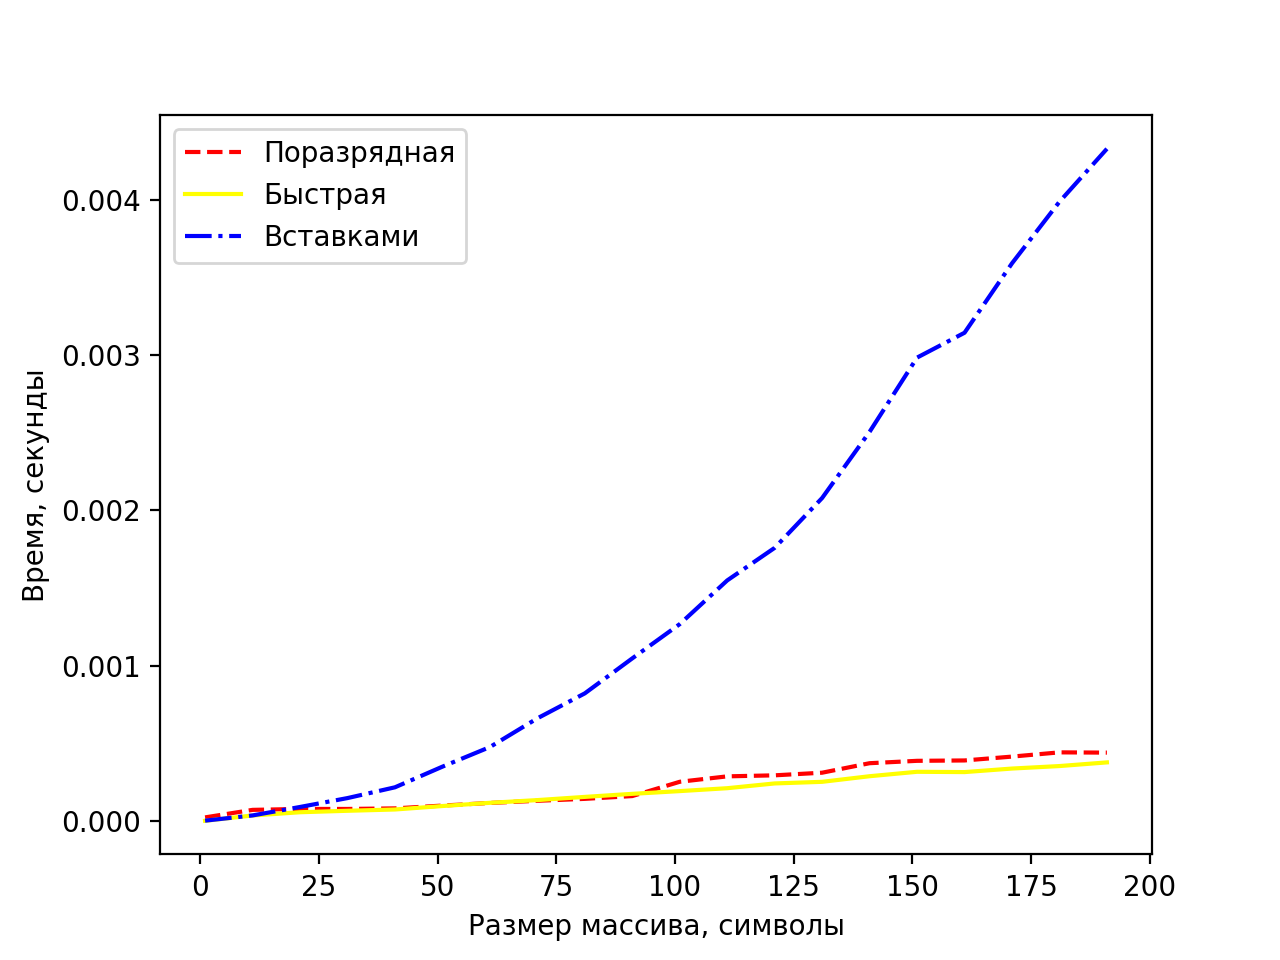
\includegraphics[scale = 1]{./pictures/graph6} \\ Рис. 4.9 - Сравнение реализации алгоритмов сортировок на обратно упорядоченных данных.
	\end{center}
	\begin{center}
        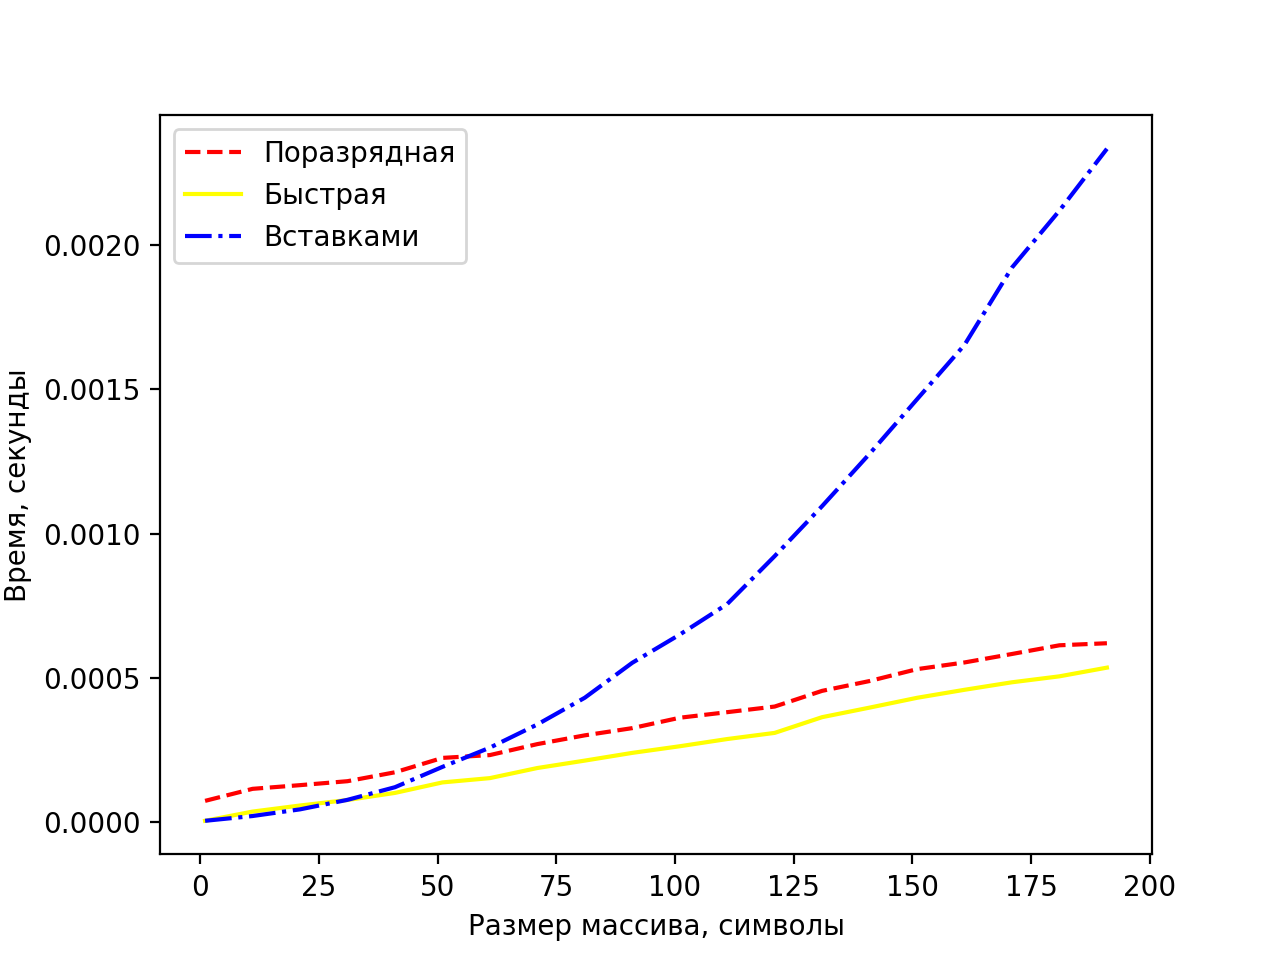
\includegraphics[scale = 1]{./pictures/graph7} \\ Рис. 4.10 - Сравнение реализации алгоритмов сортировок на произвольных данных при небольших размерах
        массивов.
	\end{center}
\section{Выводы}
Как видно из графиков и из проведенного анализа трудоемкости, поразрядная сортировка имеет
линейную зависимость от длины массива и разрядности элементов; быстрая - квадаратичную в худшем
случае и 𝑛 · 𝑙𝑜𝑔(𝑛) - в остальных; поразрядная - линейную в лучшем и квадратичную в среднем и худшем
случаях.
\pagebreak

